\documentclass[11pt,a4paper]{article}
\usepackage{fontspec}
\usepackage[polish]{babel}
\usepackage[margin=2.2cm]{geometry}
\usepackage{graphicx}
\usepackage[table]{xcolor}
\usepackage{listings}
\usepackage{tikz}
\usetikzlibrary{arrows.meta,automata,positioning}
\usepackage{amsmath}
\usepackage{booktabs}
\usepackage{caption}
\usepackage{float}
\usepackage{enumitem}
\usepackage{fancyhdr}
\usepackage[hidelinks]{hyperref}

\definecolor{pwr}{HTML}{A4161A}
\definecolor{kod}{HTML}{F6F6F6}

\lstset{
  language=VHDL,
  basicstyle=\ttfamily\small,
  keywordstyle=\color{pwr}\bfseries,
  commentstyle=\color{gray}\itshape,
  backgroundcolor=\color{kod},
  frame=single, rulecolor=\color{gray!40},
  numbers=left, numberstyle=\tiny\color{gray},
  breaklines=true, columns=fullflexible, keepspaces=true,
  xleftmargin=1.5em, framexleftmargin=1.5em
}

\captionsetup{font=small,labelfont=bf}
\setlength{\parindent}{0pt}
\setlength{\parskip}{0.6em}
\setlength{\headheight}{14pt}

\pagestyle{fancy}
\fancyhf{}
\lhead{\small UCiSW 1, laboratorium 3}
\rhead{\small Korwin, Kasiarz}
\cfoot{\thepage}

\tikzset{
  fsm/.style={>={Stealth[length=2mm]},node distance=1.3cm,font=\small,
    every state/.style={draw,thick,fill=pwr!8,minimum size=1.05cm,inner sep=1pt},
    every edge/.style={draw,->},
    lbl/.style={font=\scriptsize,fill=white,inner sep=1pt}},
  bus/.style={draw},
}

\begin{document}

\begin{titlepage}
\centering

\includegraphics[width=3.2cm]{img/pwr_logo.png}\par\vspace{0.8cm}
{\Large\bfseries Politechnika Wrocławska}\par\vspace{2.5cm}
{\large Układy Cyfrowe i Systemy Wbudowane 1}\par\vspace{0.3cm}
{\large Laboratorium}\par\vspace{1.2cm}
{\color{pwr}\rule{0.6\textwidth}{0.8pt}}\par\vspace{0.5cm}
{\LARGE\bfseries Sprawozdanie z laboratorium 3}\par\vspace{0.4cm}
{\Large Detektor sekwencji jako automat Moore'a i Mealy'ego}\par\vspace{0.2cm}
{\large wariant c): sekwencja \texttt{100100}}\par\vspace{0.5cm}
{\color{pwr}\rule{0.6\textwidth}{0.8pt}}\par
\vfill
\begin{tabular}{ll}
\textbf{Wykonali:} & Adam Korwin, 284455\\
                   & Dawid Kasiarz, 284541\\[6pt]
\textbf{Prowadzący:} & dr inż. Jarosław Sugier\\[6pt]
\textbf{Data zajęć:} & 19.11.2026
\end{tabular}
\vspace{1.5cm}
\end{titlepage}

\section{Treść zadania}

Celem ćwiczenia było zaprojektowanie detektora sześciobitowej sekwencji podawanej szeregowo na wejście \texttt{X}. W wariancie c) wykrywana sekwencja to \texttt{100100} (najpierw lewy bit). Wyjście \texttt{Y} przyjmuje wartość 1, gdy ostatnie sześć bitów wczytanych z wejścia tworzy tę sekwencję. Detektor ma wejście zegara \texttt{Clk}, wejście zezwolenia \texttt{CE} i reset \texttt{Rst}. Kolejne wystąpienia sekwencji mogą na siebie zachodzić. Ćwiczenie składało się z trzech zadań:

\begin{description}[leftmargin=2.2em,style=sameline]
  \item[Z1] detektor jako automat Moore'a: graf o $6 + 1$ stanach, w kodzie trzy przerzutniki typu D z biblioteki UNISIM i funkcja przejść zapisana tabelą \texttt{with \dots\ select}, symulacja behawioralna dla ciągu \texttt{*** abcdef *** abcdef\ensuremath{'} ***} (wektor 21-bitowy i pętla \texttt{for}) przy $f_{CLK} = 50$~MHz i czasie ustawienia wejścia \texttt{X} przed zboczem zegara równym 8~ns, ze śledzeniem wewnętrznego sygnału \texttt{Q(2:0)}; następnie implementacja jako diagram blokowy: zegar 100~MHz, dzielnik do 1~Hz, \texttt{X} z przycisku PB2, \texttt{CE} z przełącznika SW0, \texttt{Rst} z przycisku PB3, \texttt{Y} na diodzie LED0, zegar 1~Hz na diodzie LED7;
  \item[Z2] ten sam detektor opisany szablonem automatu z trzema procesami, do pokazania tylko symulacja behawioralna ze śledzeniem sygnału \texttt{state};
  \item[Z3] detektor z Z2 w wersji automatu Mealy'ego (nowy graf, 6 stanów).
\end{description}

\section{Z1: automat Moore'a}

\subsection{Graf automatu}

Stan $S_k$ oznacza, że ostatnie $k$ wczytanych bitów jest zgodne z pierwszymi $k$ bitami sekwencji. Stan $S_0$ oznacza brak dopasowania, a $S_6$ oznacza, że wczytano całą sekwencję \texttt{100100}. W automacie Moore'a wyjście zależy tylko od stanu, dlatego potrzebny jest osobny stan $S_6$, w którym $Y = 1$. Daje to sześć stanów opisujących postęp i jeden stan wykrycia, razem siedem.

Gdy przychodzi bit niezgodny z sekwencją, automat nie zawsze wraca do $S_0$. Przechodzi do stanu odpowiadającego najdłuższej końcówce wczytanego ciągu, która jest jednocześnie początkiem sekwencji \texttt{100100}:
\begin{itemize}[itemsep=0pt]
  \item w stanach $S_2$, $S_4$ i $S_5$ jedynka kończy ciąg na \texttt{1}, więc automat przechodzi do $S_1$;
  \item w stanie $S_3$ (\texttt{100}) zero daje \texttt{1000}, którego żadna końcówka nie pasuje, więc automat wraca do $S_0$;
  \item w stanie $S_6$ jedynka daje ciąg kończący się na \texttt{1001}, więc automat przechodzi do $S_4$, a zero daje \texttt{1000} i powrót do $S_0$. Przejście $S_6 \to S_4$ realizuje wykrywanie zachodzących na siebie sekwencji.
\end{itemize}

\begin{figure}[H]
\centering
\begin{tikzpicture}[fsm]
  \node[state] (s0) {$S_0/0$};
  \node[state,right=of s0] (s1) {$S_1/0$};
  \node[state,right=of s1] (s2) {$S_2/0$};
  \node[state,right=of s2] (s3) {$S_3/0$};
  \node[state,right=of s3] (s4) {$S_4/0$};
  \node[state,right=of s4] (s5) {$S_5/0$};
  \node[state,right=of s5,fill=pwr!30] (s6) {$S_6/1$};
  \path (s0) edge node[above,lbl]{1} (s1)
        (s1) edge node[above,lbl]{0} (s2)
        (s2) edge node[above,lbl]{0} (s3)
        (s3) edge node[above,lbl]{1} (s4)
        (s4) edge node[above,lbl]{0} (s5)
        (s5) edge node[above,lbl]{0} (s6)
        (s0) edge[loop above] node[lbl]{0} ()
        (s1) edge[loop above] node[lbl]{1} ()
        (s6) edge[bend right=35,pwr,thick] node[above,lbl]{1} (s4)
        (s2) edge[bend left=40] node[below,lbl]{1} (s1);
  \draw[->,gray!70!black] (s4.-100) .. controls +(-100:1.7) and +(-50:1.7) .. node[lbl,pos=0.12]{1} (s1.-50);
  \draw[->,gray!70!black] (s5.-100) .. controls +(-100:2.4) and +(-80:2.4) .. node[lbl,pos=0.1]{1} (s1.-80);
  \draw[->,violet] (s3.-100) .. controls +(-100:1.1) and +(-60:1.1) .. node[lbl,pos=0.15]{0} (s0.-60);
  \draw[->,violet] (s6.-100) .. controls +(-100:3.1) and +(-90:3.1) .. node[lbl,pos=0.08]{0} (s0.-90);
\end{tikzpicture}
\caption{Graf automatu Moore'a. Etykieta strzałki to wartość $X$, w kółku podano stan i wartość $Y$. Szare strzałki: jedynka cofa do $S_1$, fioletowe: zero cofa do $S_0$. Wyróżniono stan wykrycia i przejście $S_6 \to S_4$.}
\label{fig:graf_moore}
\end{figure}

\subsection{Kodowanie stanów i tabela przejść}

Siedem stanów wymaga trzech bitów, czyli trzech przerzutników. Zastosowaliśmy naturalne kodowanie binarne: numer stanu jest jego kodem $Q_2Q_1Q_0$. Kod \texttt{111} nie jest używany. Przerzutnik D przy narastającym zboczu przepisuje wejście na wyjście, więc wzbudzenia $D_2D_1D_0$ są po prostu kodem stanu następnego.

\begin{table}[H]
\centering
\small
\begin{tabular}{cccccc}
\toprule
Stan & Co już pasuje & $Q_2Q_1Q_0$ & $D$ dla $X = 0$ & $D$ dla $X = 1$ & $Y$\\
\midrule
$S_0$ & -- & 000 & 000 ($S_0$) & 001 ($S_1$) & 0\\
$S_1$ & \texttt{1} & 001 & 010 ($S_2$) & 001 ($S_1$) & 0\\
$S_2$ & \texttt{10} & 010 & 011 ($S_3$) & 001 ($S_1$) & 0\\
$S_3$ & \texttt{100} & 011 & 000 ($S_0$) & 100 ($S_4$) & 0\\
$S_4$ & \texttt{1001} & 100 & 101 ($S_5$) & 001 ($S_1$) & 0\\
$S_5$ & \texttt{10010} & 101 & 110 ($S_6$) & 001 ($S_1$) & 0\\
$S_6$ & \texttt{100100} & 110 & 000 ($S_0$) & 100 ($S_4$) & \textbf{1}\\
-- & (nieużywany) & 111 & 000 ($S_0$) & 000 ($S_0$) & 0\\
\bottomrule
\end{tabular}
\caption{Tabela przejść i wyjść automatu Moore'a.}
\label{tab:moore}
\end{table}

\subsection{Opis w VHDL}

Podobnie jak w laboratorium 2 użyliśmy przerzutników \texttt{FDRE} z biblioteki UNISIM. Mają one wejście zezwolenia \texttt{CE} i synchroniczny reset \texttt{R}, więc sygnały \texttt{CE} i \texttt{Rst} detektora podłączyliśmy bezpośrednio do przerzutników i nie występują one w funkcji przejść.

Funkcję przejść zapisaliśmy instrukcją \texttt{with \dots\ select}. Wejście i stan sklejamy w czterobitowy wektor \texttt{Sel = X \& Q}, ponieważ w VHDL-93 wyrażeniem wyboru nie może być konkatenacja. Każdy wiersz instrukcji odpowiada jednej komórce tabeli~\ref{tab:moore}, na przykład \texttt{"100" when "1011"} to przejście $S_3 \to S_4$ przy $X = 1$. Wiersze dające ten sam wynik połączyliśmy znakiem \texttt{|}. Wszystkie przejścia do $S_0$, w tym ze stanu nieużywanego \texttt{111} i dla wartości \texttt{U}, \texttt{X} typu \texttt{std\_logic}, obejmuje gałąź \texttt{when others}. Wyjście $Y$ jest równe 1 tylko dla $Q = \texttt{110}$.

\lstinputlisting[caption={Plik \texttt{Detektor\_c.vhd}}]{../Detektor_c.vhd}

\subsection{Testbench}

Zegar 50~MHz ma okres $T = 1/50\,\text{MHz} = 20$~ns, więc w testbenchu sygnał \texttt{Clk} zmienia stan co 10~ns, a zbocza narastające wypadają w chwilach 10, 30, 50, \dots~ns. Wejście \texttt{X} ma się zmieniać 8~ns przed zboczem ($T_{SU} = 8$~ns), czyli $T - T_{SU} = 12$~ns po poprzednim zboczu. Proces \texttt{Stim} czeka na zbocze narastające, odczekuje 12~ns i podaje kolejny bit wektora.

Wektor 21-bitowy ma postać
\[
\underbrace{000}_{***}\;\underbrace{100100}_{abcdef}\;\underbrace{000}_{***}\;\underbrace{100101}_{abcdef'}\;\underbrace{000}_{***}.
\]
Pierwsza szóstka jest szukaną sekwencją i ma dać jedno wykrycie. W drugiej szóstce ostatni bit jest zanegowany, więc wykrycia być nie powinno. Reset jest aktywny do chwili 22~ns, tak aby pierwsze zbocze ustawiło automat w stanie $S_0$.

\lstinputlisting[caption={Plik \texttt{Detektor\_tb.vhd}}]{../Detektor_tb.vhd}

\subsection{Wynik symulacji}

Na wykres dodaliśmy wewnętrzny sygnał \texttt{Q[2:0]} z instancji \texttt{UUT} (zakładka \emph{Scope}, następnie \emph{Objects}, \emph{Add to Wave Window}) i ponownie uruchomiliśmy symulację poleceniami \texttt{restart} i \texttt{run}. Przebieg przedstawia rysunek~\ref{fig:sim_z1}.

\begin{figure}[H]
\centering
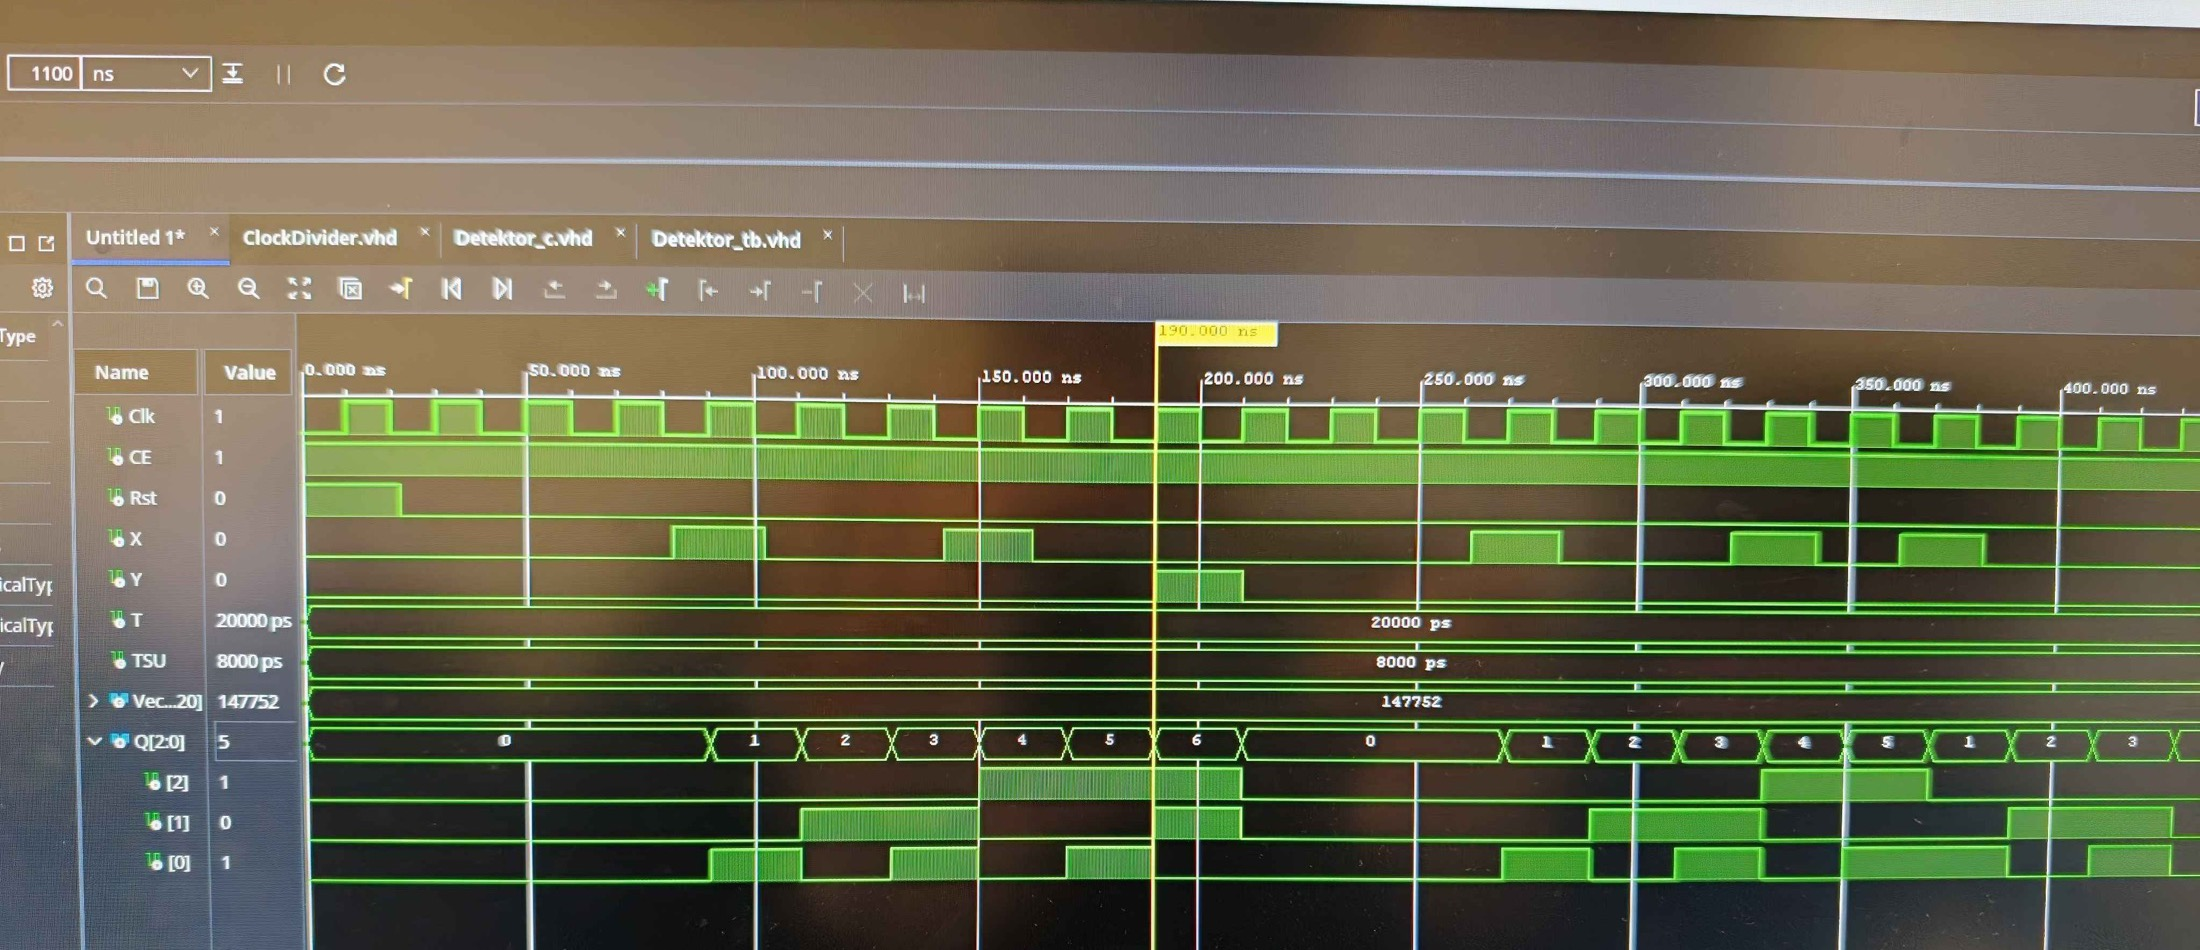
\includegraphics[width=\textwidth]{img/sim_z1.jpg}
\caption{Symulacja behawioralna automatu Moore'a w Vivado (zdjęcie ekranu z zajęć). Szyna \texttt{Q[2:0]} jest pokazana dziesiętnie, pod nią bity $Q(2)$, $Q(1)$, $Q(0)$. Kursor ustawiono w chwili 190~ns.}
\label{fig:sim_z1}
\end{figure}

Stan automatu zmieniał się w kolejności
\[
0,\ 0,\ 0,\ 1,\ 2,\ 3,\ 4,\ 5,\ \mathbf{6},\ 0,\ 0,\ 0,\ 1,\ 2,\ 3,\ 4,\ 5,\ 1,\ 2,\ 3,\ 0,
\]
zgodnie z tabelą~\ref{tab:moore}. Wyjście $Y$ przyjęło wartość 1 dokładnie raz, w przedziale 190--210~ns, gdy automat był w stanie $S_6$. Druga szóstka (\texttt{100101}) doprowadziła automat do stanu $S_5$, a ostatnia jedynka cofnęła go do $S_1$, więc $Y$ pozostało równe 0. Widać też, że $Y$ zmienia się wyłącznie na zboczach zegara, razem ze stanem.

\subsection{Implementacja jako diagram blokowy}

W tym samym projekcie utworzyliśmy diagram blokowy z modułami RTL \texttt{Detektor} i \texttt{ClockDivider} (od prowadzącego, parametry \texttt{IN\_FREQ\_HZ} = 100E6, \texttt{OUT\_FREQ\_HZ} = 1). Zegar 100~MHz dostarcza blok \emph{Clocking Wizard} podłączony do różnicowego zegara płyty, bez wejścia \texttt{reset} i wyjścia \texttt{locked}. Wyjście dzielnika taktuje detektor i jest jednocześnie wyprowadzone na port \texttt{Clk\_1Hz}. Gotowy diagram przedstawia rysunek~\ref{fig:bd_z1}.

\begin{figure}[H]
\centering
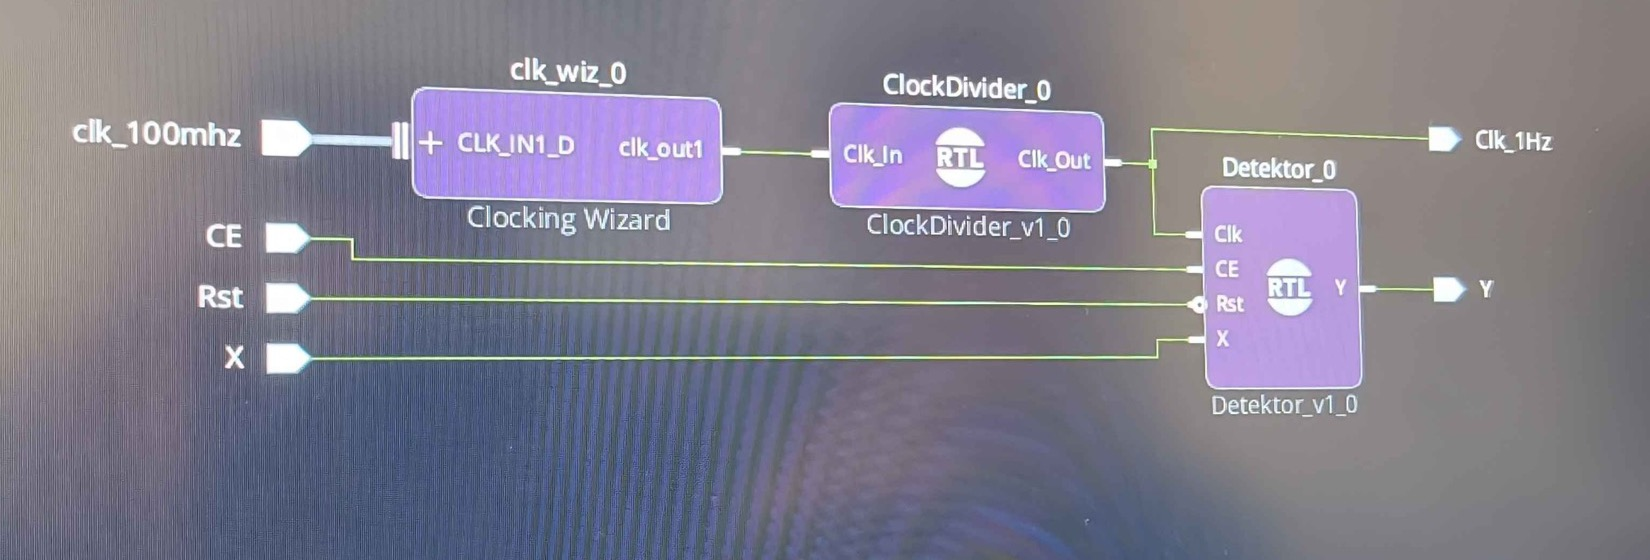
\includegraphics[width=0.85\textwidth]{img/bd_z1.jpg}
\caption{Diagram blokowy zadania Z1 (zdjęcie ekranu z zajęć).}
\label{fig:bd_z1}
\end{figure}

Numery wyprowadzeń wzięliśmy z pliku \texttt{ZU3.xdc}. Przyciski PB0--PB3 z tego pliku to przyciski oznaczone na płycie jako BTN0--BTN3. Linii zegara w pliku XDC nie ma, ponieważ opisuje go \emph{Clocking Wizard}.

\lstinputlisting[language={},caption={Plik \texttt{Z1.xdc}}]{../Z1.xdc}

Na płycie detektor jest taktowany zegarem 1~Hz, więc wczytuje jeden bit na sekundę, w chwili zapalenia diody LD7. Bit podaje się przyciskiem PB2: wciśnięty oznacza 1, puszczony 0. Stan przycisku należy zmieniać w czasie, gdy LD7 świeci, aby przy następnym zboczu był już ustalony. Sposób sprawdzenia przedstawia tabela~\ref{tab:plyta}.

\begin{table}[H]
\centering
\small
\begin{tabular}{p{7.6cm}p{6.4cm}}
\toprule
Czynność (SW0 = 1) & Oczekiwany stan LD0\\
\midrule
PB3 przez jedno mignięcie LD7, następnie PB2 kolejno: wciśnięty, puszczony, puszczony, wciśnięty, puszczony, puszczony (\texttt{100100}) & zapala się przy szóstym mignięciu i świeci 1~s\\
Dalej PB2: wciśnięty, puszczony, puszczony (\texttt{100}) & zapala się ponownie (przejście $S_6 \to S_4$)\\
Ciąg \texttt{100101} & nie zapala się\\
SW0 = 0 & automat stoi, przyciski nie zmieniają stanu\\
\bottomrule
\end{tabular}
\caption{Test detektora na płycie.}
\label{tab:plyta}
\end{table}

\section{Z2: szablon automatu z trzema procesami}

W drugiej wersji opisaliśmy ten sam automat Moore'a bez przerzutników z biblioteki i bez ręcznego kodowania stanów. Stany są wartościami typu wyliczeniowego \texttt{state\_type}, a opis składa się z trzech procesów:
\begin{itemize}[itemsep=0pt]
  \item \texttt{reg}: rejestr stanu, jedyny proces synchroniczny. Na zboczu narastającym przy \texttt{Rst} = 1 ustawia stan $S_0$, w przeciwnym razie przy \texttt{CE} = 1 przepisuje \texttt{next\_state} do \texttt{state}. Odpowiada trzem przerzutnikom \texttt{FDRE} z Z1;
  \item \texttt{nxt}: funkcja przejść, proces kombinacyjny z listą czułości \texttt{(state, X)}. Instrukcja \texttt{case} ma po jednej gałęzi na stan, a każda gałąź zawiera dwie strzałki grafu z rysunku~\ref{fig:graf_moore}. Odpowiada tabeli \texttt{with \dots\ select} z Z1;
  \item \texttt{outp}: funkcja wyjścia, proces kombinacyjny zależny tylko od \texttt{state}, ponieważ jest to automat Moore'a.
\end{itemize}

Kodowanie stanów wybiera narzędzie syntezy. Ponieważ ta wersja definiuje encję o tej samej nazwie \texttt{Detektor}, umieściliśmy ją w osobnym projekcie.

\lstinputlisting[caption={Plik \texttt{Detektor\_c\_fsm.vhd}}]{../Detektor_c_fsm.vhd}

Do symulacji użyliśmy tego samego testbencha co w Z1. Na wykres dodaliśmy wewnętrzny sygnał \texttt{state}, który symulator wyświetla nazwami stanów (rysunek~\ref{fig:sim_z2}).

\begin{figure}[H]
\centering
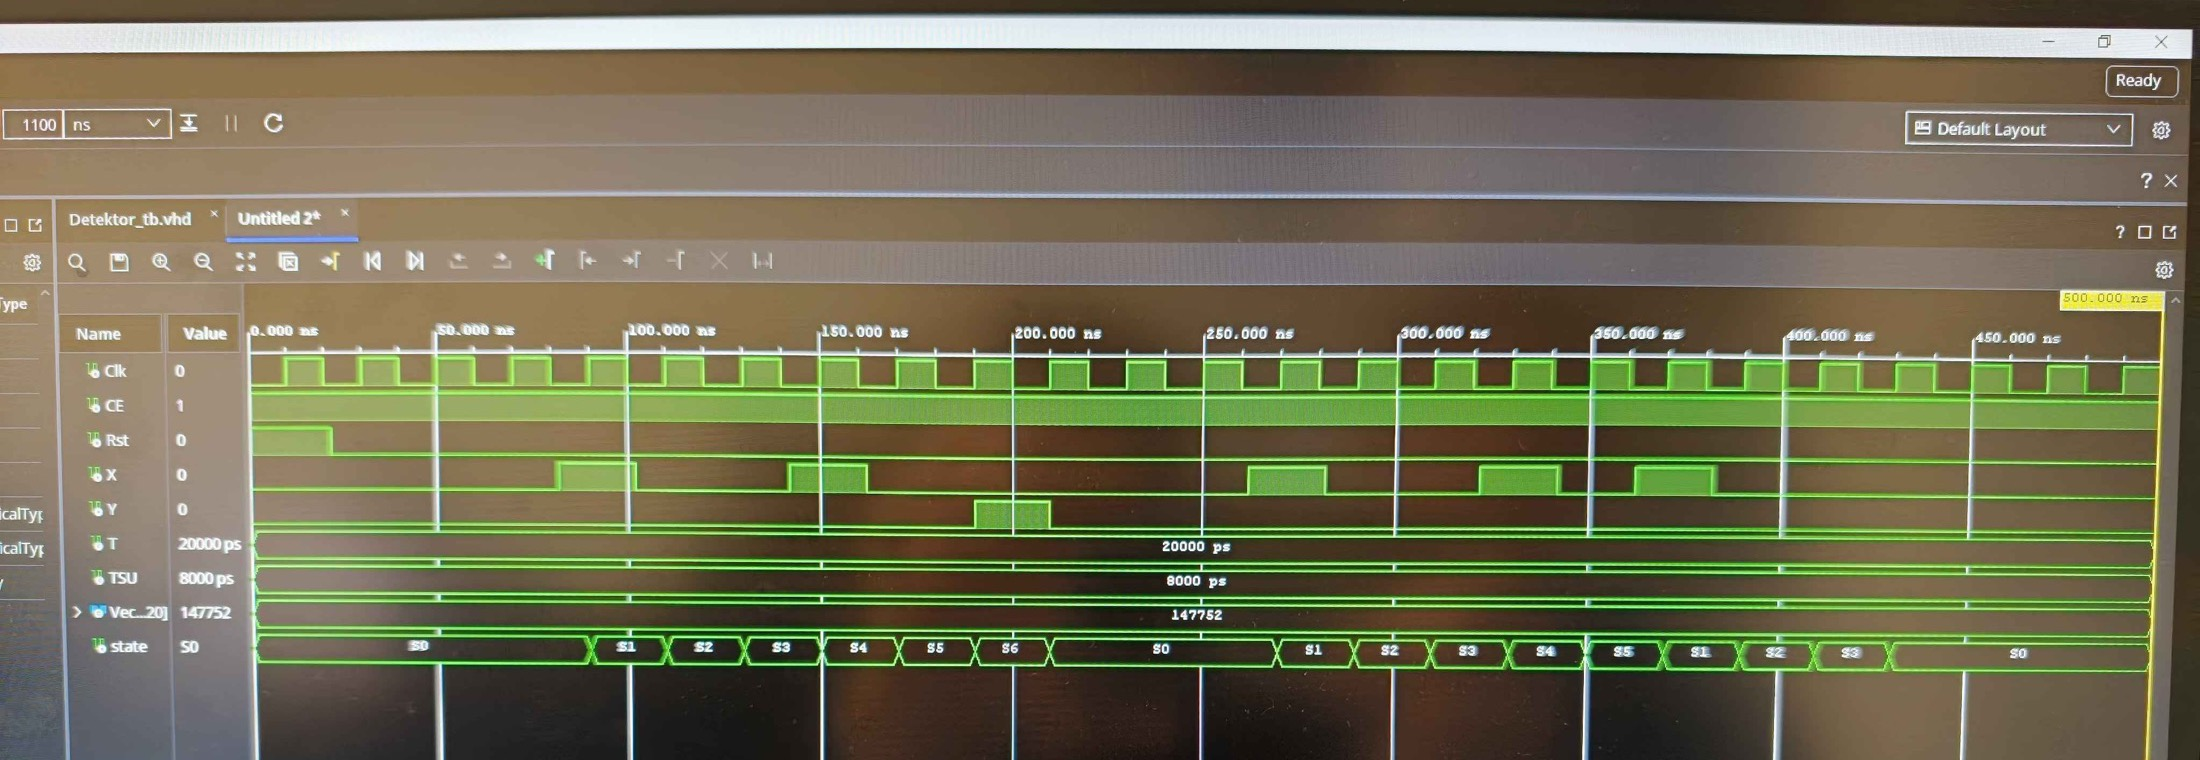
\includegraphics[width=0.88\textwidth]{img/sim_z2.jpg}
\caption{Symulacja behawioralna wersji z trzema procesami (zdjęcie ekranu z zajęć). Sygnał \texttt{state} pokazuje nazwy stanów.}
\label{fig:sim_z2}
\end{figure}

Sygnał \texttt{state} przechodził przez te same stany co \texttt{Q} w Z1: $S_0, S_1, \dots, S_6$ dla pierwszej szóstki, a dla drugiej $S_1, \dots, S_5$, powrót do $S_1$, następnie $S_2$, $S_3$, $S_0$. Wyjście $Y$ przyjęło wartość 1 tylko w przedziale 190--210~ns. Przebiegi \texttt{Clk}, \texttt{X} i \texttt{Y} są identyczne jak w Z1, co potwierdza, że obie wersje opisują ten sam automat.

\section{Z3: automat Mealy'ego}

\subsection{Graf i tabela przejść}

W automacie Mealy'ego wyjście zależy od stanu i od bieżącej wartości wejścia, więc stan wykrycia nie jest potrzebny. Wystarczy, że automat jest w stanie $S_5$ (\texttt{10010}), a na wejściu jest ostatnie zero sekwencji: wtedy $Y = 1$. Po wczytaniu tego zera ciąg kończy się na \texttt{100}, czyli pasują trzy pierwsze bity następnej sekwencji, dlatego automat przechodzi do $S_3$. Stan $S_3$ ma dokładnie te same przejścia, które w automacie Moore'a miał stan $S_6$ (zero do $S_0$, jedynka do $S_4$), więc zachodzące na siebie sekwencje są nadal wykrywane. Pozostałe przejścia są takie same jak w Z1.

\begin{figure}[H]
\centering
\begin{tikzpicture}[fsm,node distance=1.85cm]
  \node[state] (s0) {$S_0$};
  \node[state,right=of s0] (s1) {$S_1$};
  \node[state,right=of s1] (s2) {$S_2$};
  \node[state,right=of s2] (s3) {$S_3$};
  \node[state,right=of s3] (s4) {$S_4$};
  \node[state,right=of s4] (s5) {$S_5$};
  \path (s0) edge node[above,lbl]{1/0} (s1)
        (s1) edge node[above,lbl]{0/0} (s2)
        (s2) edge node[above,lbl]{0/0} (s3)
        (s3) edge node[above,lbl]{1/0} (s4)
        (s4) edge node[above,lbl]{0/0} (s5)
        (s0) edge[loop above] node[lbl]{0/0} ()
        (s1) edge[loop above] node[lbl]{1/0} ()
        (s5) edge[bend right=40,pwr,thick] node[above,lbl]{\textbf{0/1}} (s3)
        (s2) edge[bend left=40] node[below,lbl]{1/0} (s1);
  \draw[->,gray!70!black] (s4.-100) .. controls +(-100:1.8) and +(-50:1.8) .. node[lbl,pos=0.12]{1/0} (s1.-50);
  \draw[->,gray!70!black] (s5.-100) .. controls +(-100:2.6) and +(-80:2.6) .. node[lbl,pos=0.1]{1/0} (s1.-80);
  \draw[->,violet] (s3.-100) .. controls +(-100:1.2) and +(-70:1.2) .. node[lbl,pos=0.15]{0/0} (s0.-70);
\end{tikzpicture}
\caption{Graf automatu Mealy'ego. Etykieta strzałki ma postać $X/Y$. Wyróżniono jedyne przejście, w którym $Y = 1$.}
\label{fig:graf_mealy}
\end{figure}

\begin{table}[H]
\centering
\small
\begin{tabular}{cccc}
\toprule
Stan & Co już pasuje & $X = 0$ & $X = 1$\\
\midrule
$S_0$ & -- & $S_0$ / 0 & $S_1$ / 0\\
$S_1$ & \texttt{1} & $S_2$ / 0 & $S_1$ / 0\\
$S_2$ & \texttt{10} & $S_3$ / 0 & $S_1$ / 0\\
$S_3$ & \texttt{100} & $S_0$ / 0 & $S_4$ / 0\\
$S_4$ & \texttt{1001} & $S_5$ / 0 & $S_1$ / 0\\
$S_5$ & \texttt{10010} & \cellcolor{pwr!18}$S_3$ / \textbf{1} & $S_1$ / 0\\
\bottomrule
\end{tabular}
\caption{Tabela przejść i wyjść automatu Mealy'ego. W komórce: stan następny / $Y$.}
\label{tab:mealy}
\end{table}

\subsection{Opis w VHDL}

Kod powstał z wersji z Z2 przez cztery zmiany: usunięcie stanu $S_6$ z typu wyliczeniowego, usunięcie gałęzi \texttt{when S6}, zmianę przejścia $S_5 \xrightarrow{0} S_6$ na $S_5 \xrightarrow{0} S_3$ oraz zmianę procesu wyjścia. Proces \texttt{outp} ma teraz na liście czułości także \texttt{X}, a warunek $Y = 1$ to \texttt{state = S5 and X = '0'}.

\lstinputlisting[caption={Plik \texttt{Detektor\_c\_mealy.vhd}}]{../Detektor_c_mealy.vhd}

Do symulacji użyliśmy tych samych pobudzeń co w Z1 i Z2: zegar 50~MHz, ten sam wektor 21-bitowy i zmiana \texttt{X} 8~ns przed zboczem. Plik \texttt{Detektor\_Mealy\_tb.vhd} różni się od \texttt{Detektor\_tb.vhd} wyłącznie nazwą encji testbencha.

\subsection{Wynik symulacji}

Rysunek~\ref{fig:sim_z3} przedstawia przebiegi automatu Mealy'ego. Dla porównania w ostatnim wierszu dodano wyjście automatu Moore'a z Z1.

\begin{figure}[H]
\centering
\begin{tikzpicture}[x=0.0285cm,y=1cm,font=\scriptsize]
  \fill[pwr!10] (170,-1.45) rectangle (190,3.45);
  \fill[gray!15] (350,-1.45) rectangle (362,3.45);
  \node[anchor=east] at (-5,3) {\texttt{Clk}};
  \node[anchor=east] at (-5,2) {\texttt{X}};
  \node[anchor=east] at (-5,1) {\texttt{state}};
  \node[anchor=east] at (-5,0) {\texttt{Y} (Mealy)};
  \node[anchor=east] at (-5,-1) {\texttt{Y} (Moore, Z1)};
  \foreach \t in {0,20,...,440} {
    \draw (\t,2.75) -- (\t+10,2.75) -- (\t+10,3.25) -- (\t+20,3.25) -- (\t+20,2.75);
  }
  \draw (0,1.75) -- (82,1.75) -- (82,2.25) -- (102,2.25) -- (102,1.75) -- (142,1.75) -- (142,2.25) -- (162,2.25) -- (162,1.75)
        -- (262,1.75) -- (262,2.25) -- (282,2.25) -- (282,1.75) -- (322,1.75) -- (322,2.25) -- (342,2.25) -- (342,1.75)
        -- (362,1.75) -- (362,2.25) -- (382,2.25) -- (382,1.75) -- (460,1.75);
  \foreach \a/\b/\v in {0/90/S0,90/110/S1,110/130/S2,130/150/S3,150/170/S4,170/190/S5,190/210/S3,210/270/S0,
                        270/290/S1,290/310/S2,310/330/S3,330/350/S4,350/370/S5,370/390/S1,390/410/S2,410/430/S3,430/460/S0} {
    \draw (\a,1) -- (\a+2,1.25) -- (\b-2,1.25) -- (\b,1) -- (\b-2,0.75) -- (\a+2,0.75) -- cycle;
    \node at ({(\a+\b)/2},1) {\v};
  }
  \draw[pwr,thick] (0,-0.25) -- (170,-0.25) -- (170,0.25) -- (190,0.25) -- (190,-0.25) -- (350,-0.25) -- (350,0.25) -- (362,0.25) -- (362,-0.25) -- (460,-0.25);
  \draw[thick] (0,-1.25) -- (190,-1.25) -- (190,-0.75) -- (210,-0.75) -- (210,-1.25) -- (460,-1.25);
  \draw[gray] (0,-1.65) -- (460,-1.65);
  \foreach \t in {0,50,...,450} {
    \draw[gray] (\t,-1.65) -- (\t,-1.75);
    \node[gray,below] at (\t,-1.75) {\t};
  }
\end{tikzpicture}
\caption{Przebiegi z symulacji behawioralnej automatu Mealy'ego, oś czasu w ns. Kolorem zaznaczono wykrycie (170--190~ns) oraz krótki impuls na wyjściu w chwilach 350--362~ns.}
\label{fig:sim_z3}
\end{figure}

Stany automatu zmieniały się w kolejności
\[
S_0,\ S_0,\ S_0,\ S_1,\ S_2,\ S_3,\ S_4,\ S_5,\ \mathbf{S_3},\ S_0,\ S_0,\ S_0,\ S_1,\ S_2,\ S_3,\ S_4,\ S_5,\ S_1,\ S_2,\ S_3,\ S_0,
\]
 zgodnie z tabelą~\ref{tab:mealy}. Wyjście $Y$ przyjęło wartość 1 w przedziale 170--190~ns, czyli jeden takt wcześniej niż w automacie Moore'a. Automat jest wtedy w stanie $S_5$, a na wejściu jest już ostatnie zero sekwencji. Na zboczu w chwili 190~ns automat przechodzi do $S_3$ i $Y$ wraca do 0.

W przedziale 350--362~ns na wyjściu pojawił się krótki impuls, mimo że druga szóstka (\texttt{100101}) nie jest szukaną sekwencją. Po zboczu w chwili 350~ns automat jest w stanie $S_5$, a wejście $X$ ma jeszcze przez 12~ns poprzednią wartość 0. W chwili 362~ns na wejście trafia ostatni bit drugiej szóstki (1) i $Y$ wraca do 0. Nie jest to błąd projektu, tylko właściwość automatu Mealy'ego: jego wyjście jest kombinacyjną funkcją wejścia, więc jest ważne dopiero po ustaleniu się \texttt{X}, czyli tuż przed zboczem zegara. W chwili zbocza 370~ns $Y = 0$, więc wykrycia nie ma.

\subsection{Porównanie automatów}

\begin{table}[H]
\centering
\small
\begin{tabular}{p{3.4cm}p{5.4cm}p{5.4cm}}
\toprule
 & Moore (Z1, Z2) & Mealy (Z3)\\
\midrule
Liczba stanów & 7 & 6\\
$Y$ zależy od & tylko stanu & stanu i wejścia $X$\\
Chwila wykrycia & przez cały takt po zboczu, które wczytało ostatni bit (190--210~ns) & w takcie, w którym ostatni bit jest na wejściu (170--190~ns)\\
Krótkie impulsy na $Y$ & nie występują & mogą wystąpić, gdy $X$ zmienia się w trakcie taktu\\
Stan po wykryciu & $S_6$, dalej $S_0$ lub $S_4$ & od razu $S_3$\\
\bottomrule
\end{tabular}
\caption{Porównanie detektora w wersji Moore'a i Mealy'ego.}
\end{table}

\section{Wnioski}

Kluczowym krokiem projektu detektora sekwencji jest poprawne określenie przejść po bicie niezgodnym z sekwencją. Automat nie może wtedy po prostu wracać do stanu początkowego, tylko do stanu odpowiadającego najdłuższej końcówce wczytanego ciągu, która jest początkiem sekwencji. Dla sekwencji \texttt{100100} najważniejsze okazały się przejścia $S_3 \xrightarrow{0} S_0$ oraz $S_6 \xrightarrow{1} S_4$, dzięki któremu wykrywane są zachodzące na siebie wystąpienia.

Opis z przerzutnikami \texttt{FDRE} i tabelą \texttt{with \dots\ select} pokazuje strukturę układu i wymaga ręcznego zakodowania stanów. Szablon z trzema procesami opisuje ten sam automat znacznie czytelniej: stany mają nazwy, a każda gałąź \texttt{case} odpowiada wprost jednemu węzłowi grafu. Obie wersje dały identyczne przebiegi w symulacji.

Automat Mealy'ego potrzebuje o jeden stan mniej i sygnalizuje wykrycie takt wcześniej niż automat Moore'a. Ceną jest to, że jego wyjście zależy kombinacyjnie od wejścia i może zawierać krótkie, fałszywe impulsy, co było widać w symulacji w przedziale 350--362~ns. Wyjście automatu Mealy'ego należy więc odczytywać synchronicznie, przy zboczu zegara, natomiast wyjście automatu Moore'a jest stabilne przez cały takt.

\end{document}
